\documentclass[border=10pt]{standalone}

\usepackage{tikz}
\usepackage{tikzsymbols}
\usetikzlibrary{calc,patterns,shapes.geometric}

\def\centerarc[#1](#2)(#3:#4:#5){\draw[#1] ($(#2)+({#5*cos(#3)},{#5*sin(#3)})$) arc (#3:#4:#5);}

\begin{document}
	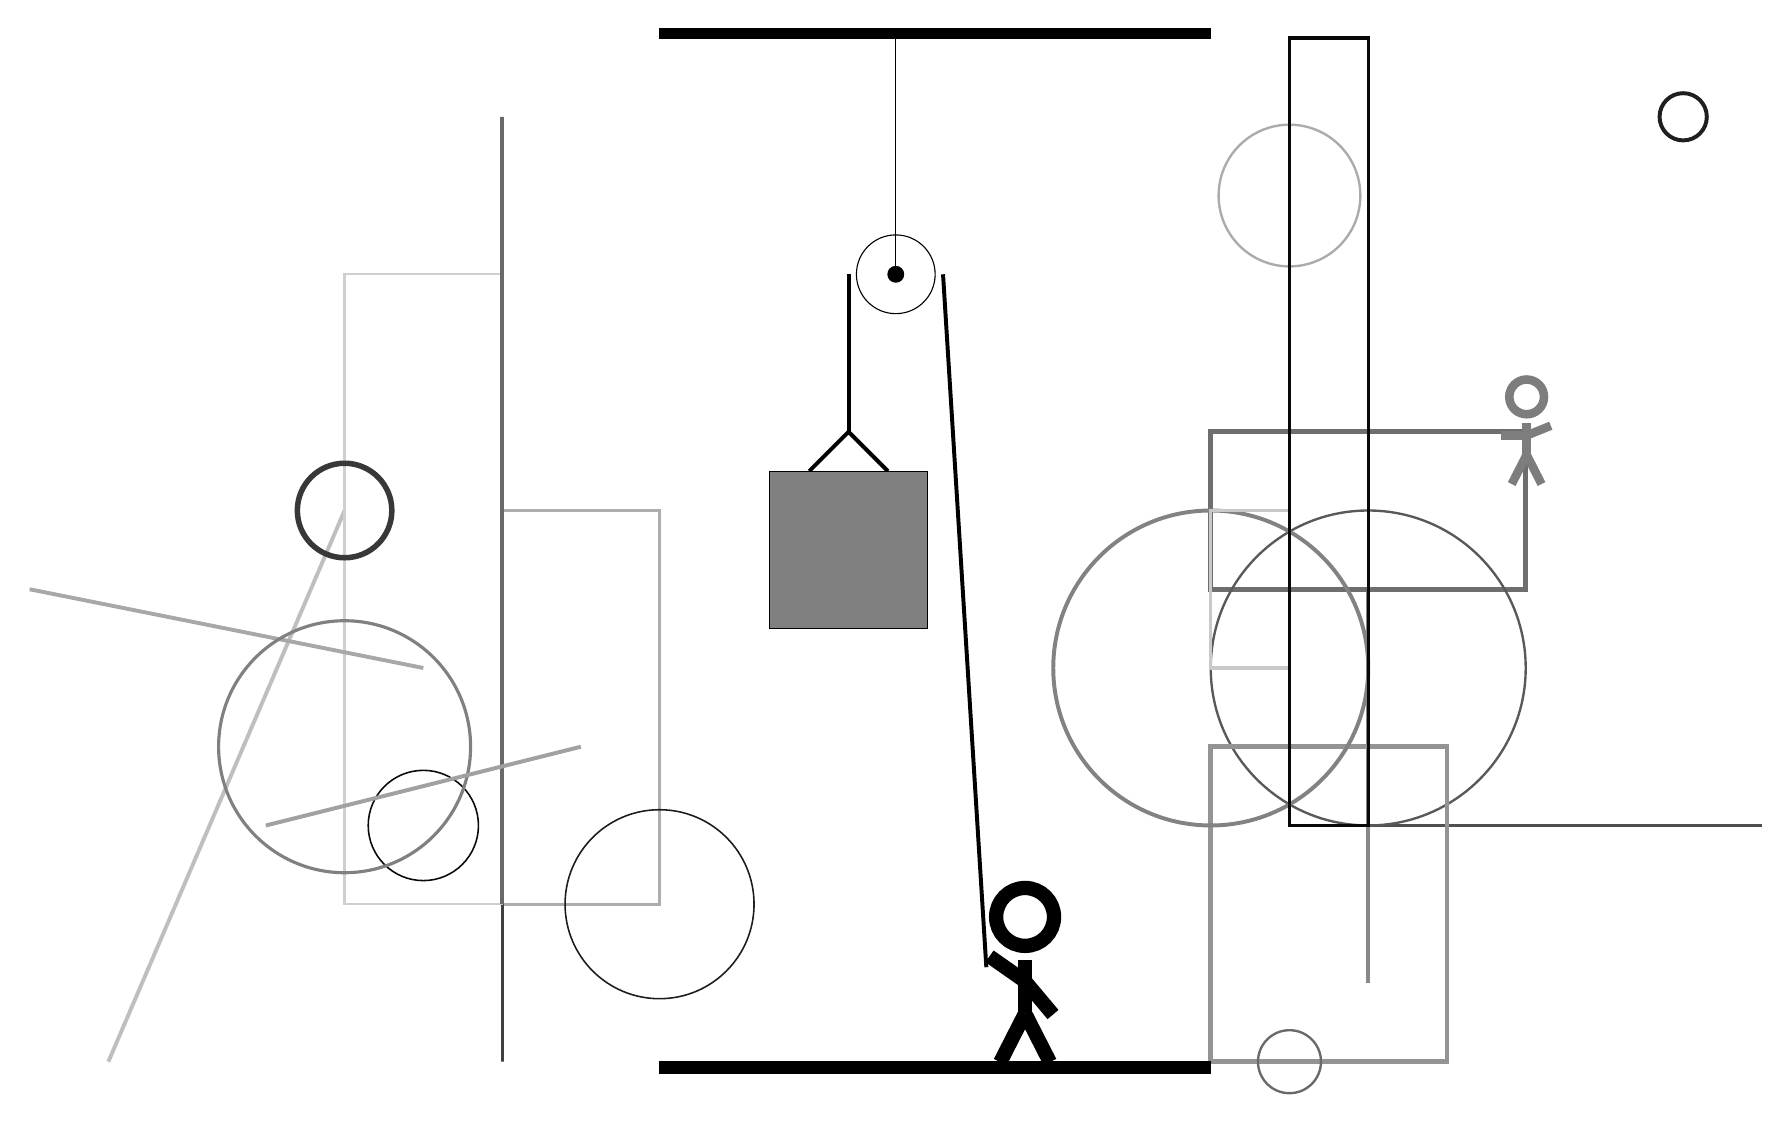
\begin{tikzpicture}
		%%%%% START %%%%%
		
		\draw[fill=black] (-2, 10) rectangle (5, 10.125);
		
		\draw (1, 7) circle (0.5);
		\draw[fill=black] (1, 7) circle (0.1);
		\draw (1, 10) -- (1, 7);
		
		\draw[line width=0.5mm] (-0.1, 4.5) -- (0.4, 5.0) -- (0.9, 4.5);
		\draw[fill=black!50] (-0.6, 4.5) rectangle (1.4, 2.5);
		
		\draw[line width=0.5mm] (0.4, 7) -- (0.4, 5.0);
		\centerarc[line width=0.5mm](1, 7)(0:180:0.6);
		\draw[line width=0.5mm](1.6, 7) -- (2.15, -1.8);
		
		\node at (2.6, -1.9) {\Strichmaxerl[10][-35][-50]};
		
		\draw [line width=0.5mm, color=black!88](11, 9) circle (0.3);
		
		\draw[line width=0.5mm, color=black!47](7, 3) -- (7, -2);
		\draw[line width=0.4mm, color=black!32] (-4, -1) rectangle (-2, 4);
		\draw[line width=0.4mm, color=black!75] (-4, -3) rectangle (-4, 8);
		\draw[line width=0.5mm, color=black!25](-6, 4) -- (-9, -3);
		\draw[line width=0.3mm, color=black!19] (-4, -1) rectangle (-6, 7);
		\draw[line width=0.5mm, color=black!59] (-4, 9) rectangle (-4, -1);
		\draw[line width=0.6mm, color=black!57] (5, 5) rectangle (9, 3);
		\node[line width=0.7mm, color=black!51] at (9, 5) {\Strichmaxerl[6][0][22]};
		
		\draw[line width=0.5mm, color=black!34](-5, 2) -- (-10, 3);
		\draw[line width=0.5mm, color=black!69](6, 0) -- (12, 0);
		
		\draw [line width=0.3mm, color=black!65](7, 2) circle (2.0);
		\draw[line width=0.6mm, color=black!42] (5, 1) rectangle (8, -3);
		
		\draw [line width=0.7mm, color=black!78](-6, 4) circle (0.6);
		\draw [line width=0.2mm, color=black!96](-5, 0) circle (0.7);
		\draw [line width=0.3mm, color=black!59](6, -3) circle (0.4);
		
		\draw [line width=0.3mm, color=black!33](6, 8) circle (0.9);
		
		\draw [line width=0.2mm, color=black!89](-2, -1) circle (1.2);
		\draw [line width=0.5mm, color=black!49](5, 2) circle (2.0);
		\draw [line width=0.4mm, color=black!50](-6, 1) circle (1.6);
		\draw[line width=0.4mm, color=black!21] (5, 4) rectangle (6, 2);
		\draw[line width=0.4mm, color=black!97] (6, 0) rectangle (7, 10);
		\draw[line width=0.5mm, color=black!37](-3, 1) -- (-7, 0);
		
		\draw[fill=black] (-2, -3) rectangle (5, -3.15);
		
		%%%%% END %%%%%
	\end{tikzpicture}
\end{document}